\section{Introduction}\label{sec:intro}

ReLU gates each neuron by its sign: $\mathrm{ReLU}(z_i) = z_i \cdot \mathbf{1}[z_i > 0]$.
This binary gate is coarse---it can only fully pass or fully block---but it has an underappreciated property: it is \emph{scale-invariant}.
Multiplying all pre-activations by any $\alpha > 0$ scales the output but leaves every gating decision, and therefore the output \emph{direction}, unchanged.

The smooth self-gated activations that have largely replaced ReLU in modern architectures---GELU~\citep{hendrycks2016gaussian} ($g{=}\Phi$, the normal CDF) and SiLU/Swish~\citep{elfwing2018sigmoid,ramachandran2017searching} ($g{=}\sigma$, the sigmoid)---share the form $f(z_i) = z_i \cdot g(z_i)$, where $g$ is a smooth monotonic gate.
They offer smoother gradients, graded modulation, and no dead neurons.
But we prove that \emph{no} non-constant smooth gate $g$ can preserve scale invariance in this form (Proposition~\ref{prop:no_invariance}): replacing ReLU's binary gate with a smooth one necessarily makes the output direction depend on absolute scale.

This is not merely a change in output magnitude.
The next layer's response decomposes as $\langle \mathbf{w}_j, \mathbf{y}\rangle = \|\mathbf{y}\| \cdot \langle \mathbf{w}_j, \hat{\mathbf{y}}\rangle$: magnitude acts as gain; all selectivity---which features the next layer responds to---comes from the direction $\hat{\mathbf{y}}$.
We do not argue that activation magnitude is uninformative; our claim is narrower: a common scale factor may reasonably modulate output magnitude, but need not alter the output direction through which downstream layers identify features.
In the self-gated form, it does both, entangling the two roles.

Figure~\ref{fig:teaser} illustrates this concretely.
Under scale perturbation $\mathbf{z} \to (1{+}\epsilon)\mathbf{z}$, ReLU's output direction is exactly invariant ($0^\circ$ rotation).
GELU's direction rotates by up to $18.8^\circ$---the same underlying pattern is mapped to a different downstream signal depending on scale.
NELU (Section~\ref{sec:method}) restores exact invariance ($0^\circ$).

\paragraph{Contributions.}
\begin{enumerate}[leftmargin=1.5em,itemsep=2pt,topsep=3pt]
    \item We prove that scale invariance is incompatible with smooth self-gating: for any non-constant $g$, the output direction of $z_i \cdot g(z_i)$ depends on absolute scale.
    We show that weight growth during training compounds this by driving the gate toward saturation, progressively reducing the graded-gating regime (Section~\ref{sec:problem}).

    \item We propose NELU (Normalized Gaussian Error Linear Unit), to our knowledge the first smooth self-gated activation with provably scale-invariant output direction (Section~\ref{sec:method}):
    \begin{equation}\label{eq:nelu_intro}
        \mathrm{NELU}(\mathbf{z})_i = z_i \;\Phi\!\left(\frac{z_i}{\operatorname{sg}[\rho]}\right), \quad \rho = \operatorname{rms}(\mathbf{z}).
    \end{equation}
    Scale is not discarded but redirected: removed from the gate, preserved in the output magnitude ($\mathrm{NELU}(\alpha\mathbf{z}) = \alpha\,\mathrm{NELU}(\mathbf{z})$).
    We provide a complete characterization: differentiability, Lipschitz continuity, boundedness, and stop-gradient analysis.

    \item NELU matches or improves GELU across CNNs (CIFAR-10/100), ViTs (ImageNet), and language models (GPT-2 up to 774M).
    On corruption benchmarks, where pre-activation scale shifts are most pronounced, NELU's advantage is largest (Section~\ref{sec:experiments}).
\end{enumerate}

%%% FIGURE: Teaser
\begin{figure}[t]
\centering
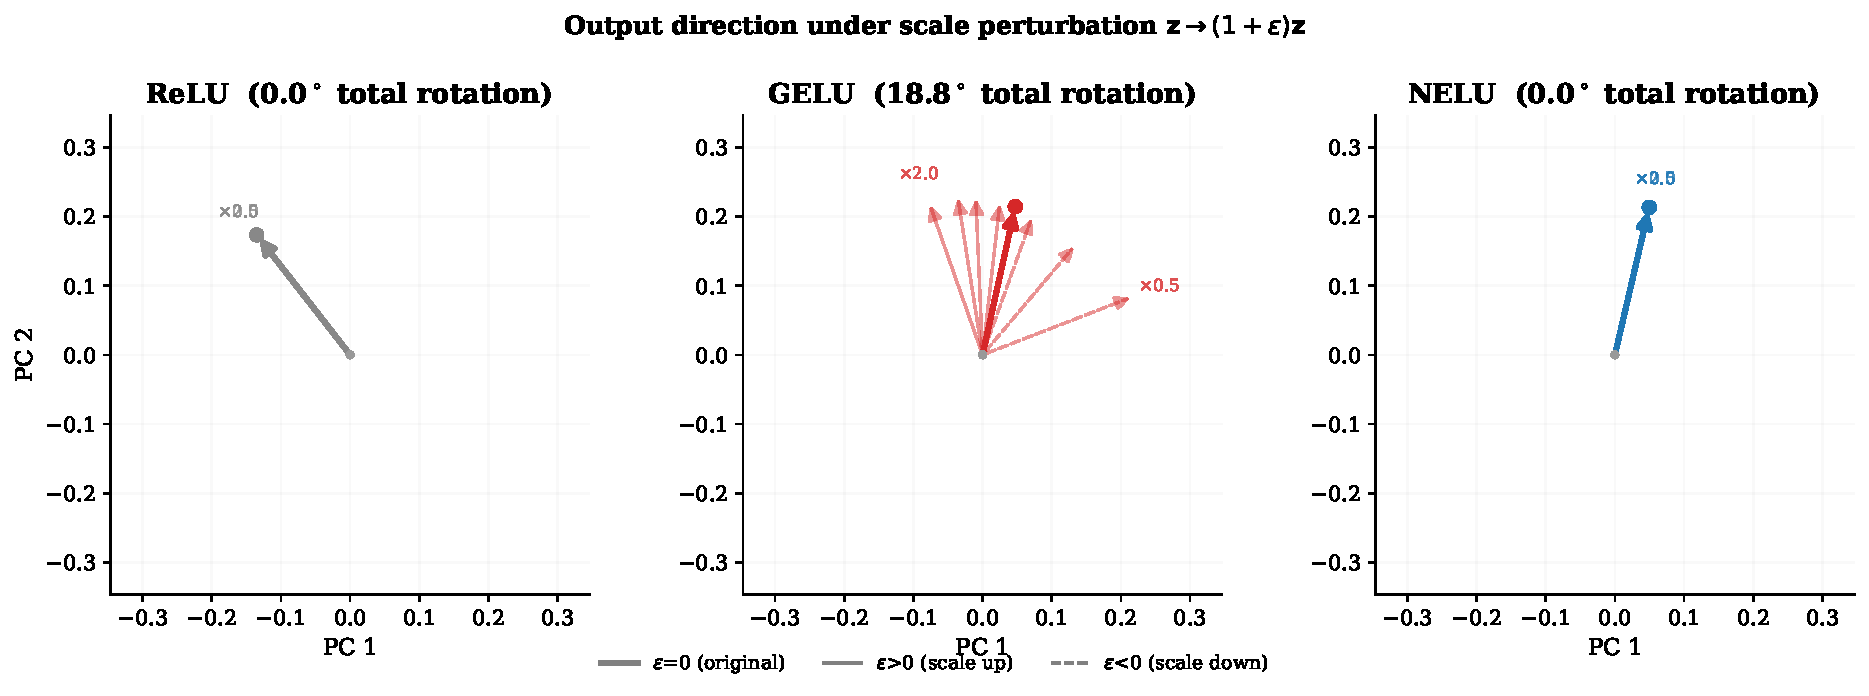
\includegraphics[width=\linewidth]{figures/fig1_teaser.pdf}
\caption{\textbf{Output direction under scale perturbation $\mathbf{z} \to (1{+}\epsilon)\mathbf{z}$.}
A random pre-activation vector $\mathbf{z} \in \mathbb{R}^{128}$ is scaled by factors $\alpha \in [0.5, 2.0]$; each arrow shows the output direction (projected via PCA) at a different $\alpha$.
\textbf{Left:}~ReLU's direction is exactly invariant ($0^\circ$ total rotation).
\textbf{Center:}~GELU's direction rotates as scale changes ($18.8^\circ$): the same feature pattern is mapped to different directions depending on absolute magnitude.
\textbf{Right:}~NELU (Section~\ref{sec:method}) restores exact invariance ($0^\circ$).}
\label{fig:teaser}
\end{figure}